% Copyright 2004 by Till Tantau <tantau@users.sourceforge.net>.
%
% In principle, this file can be redistributed and/or modified under
% the terms of the GNU Public License, version 2.
%
% However, this file is supposed to be a template to be modified
% for your own needs. For this reason, if you use this file as a
% template and not specifically distribute it as part of a another
% package/program, I grant the extra permission to freely copy and
% modify this file as you see fit and even to delete this copyright
% notice. 

\documentclass{beamer}

% There are many different themes available for Beamer. A comprehensive
% list with examples is given here:
% http://deic.uab.es/~iblanes/beamer_gallery/index_by_theme.html
% You can uncomment the themes below if you would like to use a different
% one:
%\usetheme{AnnArbor}
%\usetheme{Antibes}
%\usetheme{Bergen}
%\usetheme{Berkeley}
%\usetheme{Berlin}
%\usetheme{Boadilla}
%\usetheme{boxes}
%\usetheme{CambridgeUS}
%\usetheme{Copenhagen}
%\usetheme{Darmstadt}
%\usetheme{default}
%\usetheme{Frankfurt}
%\usetheme{Goettingen}
%\usetheme{Hannover}
%\usetheme{Ilmenau}
%\usetheme{JuanLesPins}
%\usetheme{Luebeck}
%\usetheme{Madrid}
%\usetheme{Malmoe}
%\usetheme{Marburg}
%\usetheme{Montpellier}
%\usetheme{PaloAlto}
%\usetheme{Pittsburgh}
%\usetheme{Rochester}
%\usetheme{Singapore}
%\usetheme{Szeged}
%\usetheme{Warsaw}

\usepackage{amsmath}
\usepackage{textpos}
\usepackage{ulem}
%\usepackage{enumitem}
\usepackage{bm}
\usepackage{algorithm}
\usepackage[noend]{algpseudocode}

\usepackage{amsthm}
\newtheorem{thm}{Theorem}

\usepackage{paralist}
\usepackage{comment}
\usepackage{subfigure}

\usepackage[labelformat=empty]{caption}

\definecolor{BYUblue}{RGB}{0,31,69}
\definecolor{BYUgold}{RGB}{195,163,106}
\usecolortheme[RGB={0,31,69}]{structure} % BYU Blue

\definecolor{diff-point}{RGB}{102,178,255}
\definecolor{diff-path}{RGB}{0,76,153}

\definecolor{reference_color}{RGB}{0,175,0}
\definecolor{subproblem_color}{RGB}{0,0,255}

\definecolor{metric-PR}{RGB}{200,127,0}
\definecolor{metric-NE}{RGB}{51,51,255}
\definecolor{metric-OFI}{RGB}{204,0,0}
\definecolor{metric-IRO}{RGB}{0,102,51}

\newtheorem{reference_tree}{Example}
\newtheorem{subproblem_tree}{Example}
\newenvironment<>{reference_tree}[1][]{%
  \setbeamercolor{block title example}{fg=white,bg=reference_color}%
  \begin{example}#2[#1]}{\end{example}}
\newenvironment<>{subproblem_tree}[1][]{%
  \setbeamercolor{block title example}{fg=white,bg=subproblem_color}%
  \begin{example}#2[#1]}{\end{example}}


\usetheme{Frankfurt}
\setbeamercolor*{section in head/foot}{bg=BYUblue,fg=gray!25}
\setbeamercolor*{frametitle}{bg=BYUblue!50,fg=white!25}
\setbeamercovered{transparent}
\mode<all>

\DeclareMathOperator*{\argmax}{arg\,max}

\title{From Qualitative to Quantitative: Supporting Robot Understanding in Human-Interactive Path Planning}

\subtitle{\bf [ Research Topic ] }

\author{Daqing Yi}

\institute
{
  Department of DepartComputer Science\\
  Brigham Young University
}

\date[]{} 

\addtobeamertemplate{frametitle}{}{%
\begin{textblock*}{100mm}(0.9\textwidth,-1.2cm)
\includegraphics[width=1.1cm]{figure/BYU_logo.png}
\end{textblock*}}

\begin{document}

\begin{frame}
  \titlepage
\end{frame}

\begin{frame}{Outline}{$ \null $}
  \tableofcontents
  % You might wish to add the option [pausesections]
\end{frame}

% Section and subsections will appear in the presentation overview
% and table of contents.

% Add citation in the footnote

\section{Thesis Statement}

% add outline page with current section highlighted.
\begin{frame}{Outline}{$ \null $}
	%\frametitle{Outline}{ Structure }
	\tableofcontents[currentsection]
	%\tableofcontents[currentsection,currentsubsection]
\end{frame}

\begin{frame}{Thesis Statement}{ $ \null $ }

\begin{block}{ $ \null $ }

\begin{figure}
	\centering
	\includegraphics[width=.9\linewidth]{figure/thesis_statement1}
\end{figure}

\end{block}

\begin{figure}
	\centering
	\includegraphics[width=.6\linewidth]{figure/thesis_statement1_fig}
\end{figure}

\end{frame}

\begin{frame}{Thesis Statement}{ $ \null $ }

\begin{block}{$ \null $}

\begin{figure}
	\centering
	\includegraphics[width=.9\linewidth]{figure/thesis_statement2}
\end{figure}

\end{block}

\begin{figure}
	\centering
	\includegraphics[width=.8\linewidth]{figure/thesis_statement2_fig}
\end{figure}

\end{frame}

\begin{comment}

\begin{frame}

\begin{block}{}
Understand the human command
\end{block}

\begin{block}{}
Deal with the ambiguity in human commands
\end{block}

\end{frame}

\end{comment}

\section{Path-Planning from Human Language}

% add outline page with current section highlighted.
\begin{frame}{Outline}{ $ \null $ }
	\tableofcontents[currentsection]
	%\tableofcontents[currentsection,currentsubsection]
\end{frame}

\subsection{Algorithm}

\begin{frame}{Language Understanding}{ Model Path-Planning from Human Language }

\begin{columns}
	\column{0.5\textwidth}
	\begin{figure}
		\centering
		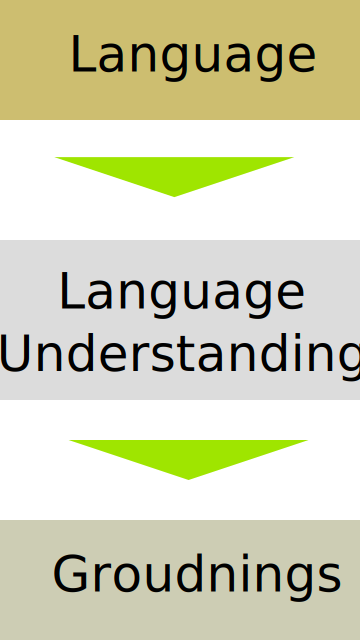
\includegraphics[width=.5\linewidth]{figure/language_understanding}
		\caption{Grounding process\footnotemark}
	\end{figure}	
	\column{0.5\textwidth}
	\begin{itemize}
	\item {\bf Phrases  $ \lambda $}

	\item {\bf Groundings $ \gamma $}
	\begin{itemize}
		\item actions
		\item landmarks / regions
		\item spatial relations
	\end{itemize}
	\end{itemize}
	
	\begin{block}{}
	\begin{equation}
	\nonumber
	\arg \max_{\gamma} P( \gamma \mid \lambda )
 	\end{equation}
 	\end{block}
 	
\end{columns}

\footnotetext[1]{\tiny {\it Tellex et al.} ``Understanding Natural Language Commands for Robotic Navigation and Mobile Manipulation.'' AAAI 2011. }

\end{frame}

\begin{frame}{Graphical Model}{ Model Path-Planning from Human Language }

\begin{columns}
\column{0.5\textwidth}
\begin{figure}
	\centering
	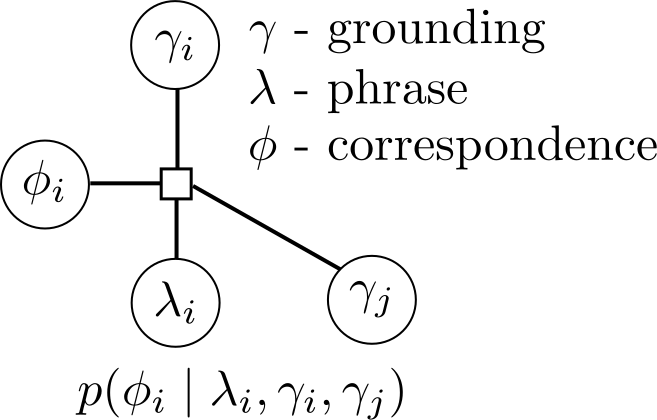
\includegraphics[width=.8\linewidth]{figure/factor_model}
\end{figure}
\column{0.5\textwidth}
\begin{itemize}
\item {\bf Correspondence $ \phi $}
\end{itemize}

\begin{block}{}
\begin{equation}
\nonumber
\arg \max_{\phi} P( \phi \mid \gamma , \lambda )
\end{equation}
\end{block}

\end{columns}

\end{frame}

\begin{frame}{Phrase Tree}{ Model Path-Planning from Human Language }

{\bf ``Move near the red box and the blue crate.''}

\begin{columns}
\column{0.5\textwidth}
\begin{figure}
	\centering
	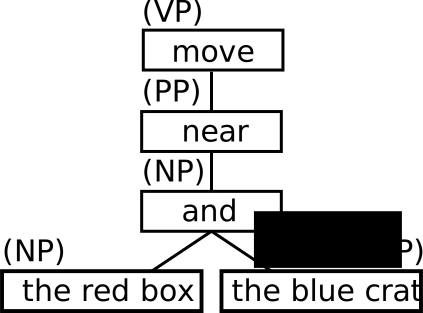
\includegraphics[width=.8\linewidth]{figure/phrase_structure2}
\end{figure}
\column{0.5\textwidth}
\begin{itemize}
\item A tree structure created by the grammar
\item Bottom-up dependencies
\end{itemize}
\end{columns}

\end{frame}

\begin{frame}{Graphical Model}{ Model Path-Planning from Human Language }

{\bf ``Move near the red box and the blue crate.''}

\begin{columns}
\column{0.5\textwidth}
\begin{figure}
	\centering
	\includegraphics[width=.9\linewidth]{figure/G3}
	\caption{ \tiny{ Howard et al. "A natural language planner interface for mobile manipulators." {\it IEEE International Conference on Robotics and Automation (ICRA) 2014.} } }
\end{figure}
\column{0.45\textwidth}
\begin{itemize}
\item Organizing factor models by the phrase tree
\end{itemize}
\end{columns}

\end{frame}

\begin{frame}{Distributed Correspondence Graph}{ Model Path-Planning from Human Language }
	
{\bf ``Move near the red box and the blue crate.''}
	
\begin{columns}
\column{0.5\textwidth}
\begin{figure}
	\centering
	\includegraphics[width=.9\linewidth]{figure/DCG}
	\caption{ \tiny{ Howard et al. "A natural language planner interface for mobile manipulators." {\it IEEE International Conference on Robotics and Automation (ICRA) 2014.} } }
\end{figure}
\column{0.45\textwidth}
\begin{itemize}
\item Train each factor model separately
\item Organize factor models into a graph model by the instruction for inference
\end{itemize}
\end{columns}

\end{frame}	

\begin{frame}{Groundings for Path-Planning}{ Model Path-Planning from Human Language } 

\begin{eqnarray}
\nonumber
\mbox{minimize: } & c(\sigma) = \int_{ \sigma } c(x) dx \\
\nonumber
\mbox{subject to: } & \sigma(0) = x_{init} \\
\nonumber
& \sigma(T) = x_{goal} \\
\nonumber
& H( \sigma(s) ) = 0 , s \in [0, T] 
\end{eqnarray}

\begin{columns}
\column{0.47\textwidth}
\begin{block}{Objective}
\begin{itemize}
\item shape of a cost function
\begin{itemize}
\item \textcolor{blue}{``avoiding ... ''}
\end{itemize}
\item types of cost functions
\begin{itemize}
\item \textcolor{blue}{``carefully ... ''}
\end{itemize}
\end{itemize}
\end{block}
\column{0.47\textwidth}
\begin{block}{Constraint}
\begin{itemize}
\item goal position / region
\begin{itemize}
\item \textcolor{blue}{``move to ... ''}
\end{itemize}
\item shapes of paths
\begin{itemize}
\item \textcolor{blue}{``by the left of ... ''}
\end{itemize}
\end{itemize}
\end{block}
\end{columns}

\end{frame}

\begin{frame}{Correspondence to the Cost Function}{ Model Path-Planning from Human Language }

{\bf Cost Function}	
	
\begin{columns}	
\column{0.3\textwidth}	
\begin{block}{World Model}
\begin{figure}
	\centering
	\includegraphics[width=.9\linewidth]{figure/world_model}
\end{figure}
\end{block}
\column{0.3\textwidth}
\begin{block}{Costmap}
\begin{figure}
	\centering
	\includegraphics[width=.9\linewidth]{figure/costmap}
\end{figure}
\end{block}
\column{0.3\textwidth}
\begin{block}{Path}
\begin{figure}
	\centering
	\includegraphics[width=.9\linewidth]{figure/costmap_path}
\end{figure}
\end{block}
\end{columns}

\begin{figure}
	\centering
	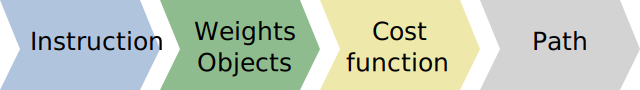
\includegraphics[width=.9\linewidth]{figure/cost_func_inference}
\end{figure}

\end{frame}

\begin{frame}{CDCG}{ Model Path-Planning from Human Language }

	\begin{itemize}
	\item {\bf Approximate the cost function by weighted sum of kernel functions}
	\begin{equation}
	\nonumber
	F( x \mid o_1 , \cdots , o_n ) = \sum_{i=1}^{n} w_i K( x \mid o_i )
	\end{equation}
	\item {\bf Ground the sentence to a cost function}
	\begin{equation}
	\nonumber
	\arg \max_{ F \in \bm{F} } p( F \mid \Lambda , \Upsilon )
	\end{equation}
	\item {\bf Continuous correspondence variables}
	\begin{equation}
	\nonumber
	\arg \max_{ w_i } \prod p'( w_i \mid \gamma_i , \lambda_i, \Gamma_{c_i} , \Upsilon )
	\end{equation}	
	\end{itemize}

\end{frame}

\begin{frame}{CDCG}{ Model Path-Planning from Human Language }
	
{\bf A mixed structure of continuous and discrete correspondence variables}
	
\begin{figure}
	\centering
	\includegraphics[width=.6\linewidth]{figure/DCG_network_structure}
\end{figure}
	
\end{frame}

\begin{frame}{HDCG}{ Model Path-Planning from Human Language }
	
	{\bf Homotopy}
	
	\begin{columns}	
	\column{0.3\textwidth}	
	\begin{block}{World Model}
	\begin{figure}
		\centering
		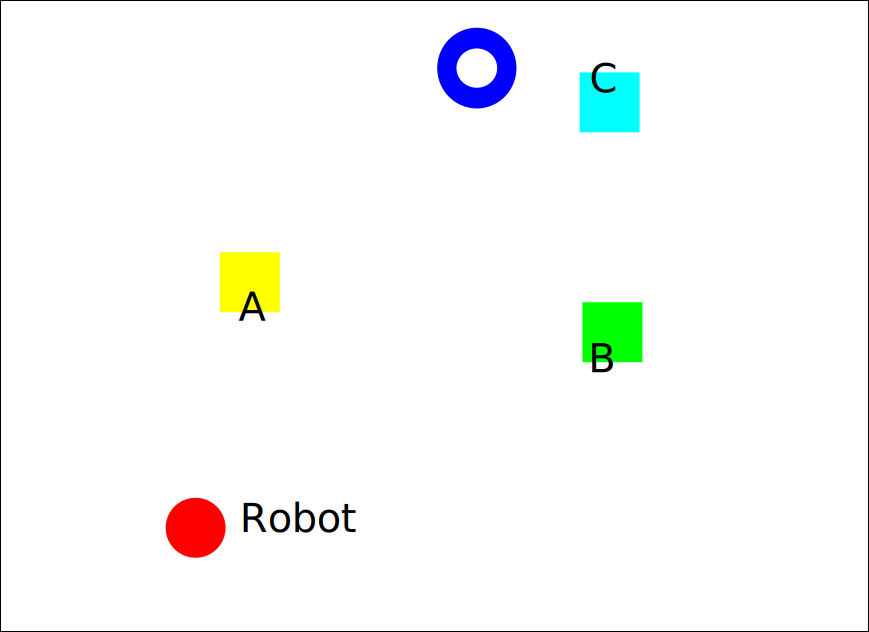
\includegraphics[width=.9\linewidth]{figure/homotopy/example_a}
	\end{figure}
	\end{block}
	\column{0.3\textwidth}
	\begin{block}{Costmap}
	\begin{figure}
		\centering
		\includegraphics[width=.9\linewidth]{figure/homotopy/example_a_decomp}
	\end{figure}
	\end{block}
	\column{0.3\textwidth}
	\begin{block}{Path}
	\begin{figure}
		\centering
		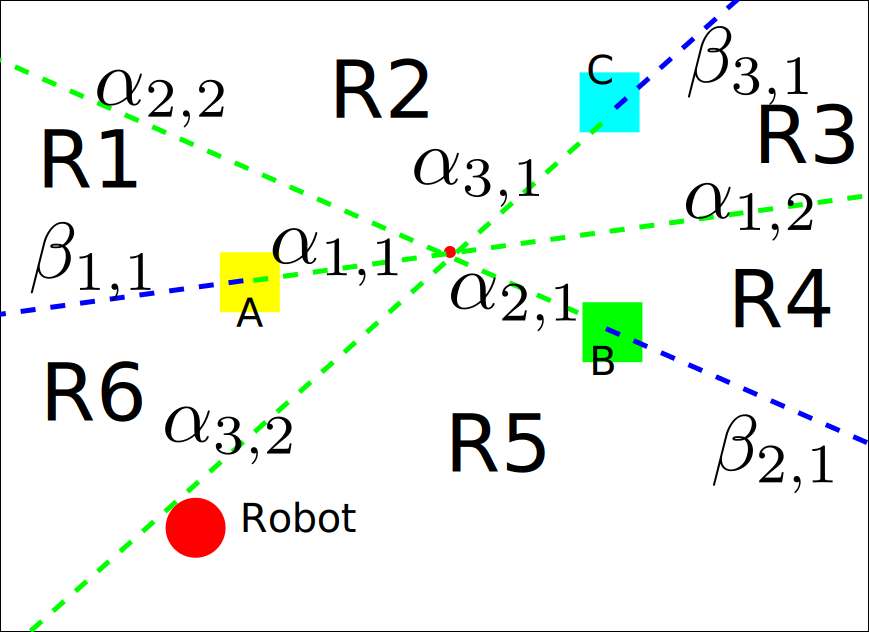
\includegraphics[width=.9\linewidth]{figure/homotopy/example_a_path}
	\end{figure}
	\end{block}
	\end{columns}
	
	\begin{figure}
		\centering
		\includegraphics[width=.9\linewidth]{figure/homotopy_inference}
	\end{figure}

\end{frame}

\begin{frame}{HDCG}{ Model Path-Planning from Human Language }

\begin{block}{Spatial relation function\footnotemark}
\begin{itemize}
\item $ R = ${\sc InBetween }$ ( \{ o_1 , o_2 \} ) $
\item $ R = ${\sc LeftOf }$ ( \{ o \} ) $ and $ R = ${\sc RightOf }$ ( \{ o \} ) $
\item $ \bar{R} = ${\sc Avoid}$ ( \{ o \} )  $
\item $ R = ${\sc Around }$ ( \{ o \} ) $
\end{itemize}
\end{block}

\begin{block}{Groundings correspond to an instruction}
\begin{itemize}
\item Objects / landmarks $ o $
\item Spatial relation functions
\end{itemize}
\end{block}

\begin{block}{Construct topological constraints}
\begin{itemize}
\item define eligible homotopy classes
\item optimal paths of eligible homotopy classes
\end{itemize}
\end{block}

\footnotetext[2]{\tiny {\it Oh et al.} ``Toward Mobile Robots Reasoning Like Humans.'' AAAI 2015.}

\end{frame}

\subsection{Validation}

\begin{frame}{Validation - Data Collection}{ Model Path-Planning from Human Language }

\begin{block}{Annotating paths}
Amazon Mechanic Turk
\end{block}

\begin{columns}	
	\column{0.6\textwidth}	
	\begin{figure}
		\centering
		\includegraphics[width=.9\linewidth]{figure/annotation_task}
	\end{figure}
	\column{0.3\textwidth}	
	\begin{figure}
		\centering
		\includegraphics[width=\linewidth]{figure/example_xml}
	\end{figure}
\end{columns}
\begin{block}{Generating example dataset}
Associate groundings with phrases
\end{block}

\end{frame}

\begin{frame}{Validation - Performance}{ Model Path-Planning from Human Language }

\begin{block}{Tranining a model with examples dataset}
Evaluate how the model fits the example dataset
\end{block}

\begin{block}{Inference using with the trained model}
Find groundings from a language instruction
\end{block}

\end{frame}






\section{Multi-Objective Path-Planning}

% add outline page with current section highlighted.
\begin{frame}{Outline}{ $ \null $ }
	\tableofcontents[currentsection]
	%\tableofcontents[currentsection,currentsubsection]
\end{frame}

\subsection{Algorithm}

\begin{frame}{Multiple Objectives in a Task}{Multi-Objective Path-Planning}
With different objectives, there are different ``best'' paths.
\begin{columns}
\column{0.45\textwidth}
	\begin{figure}
		\centering
		\includegraphics[width=.8\linewidth]{figure/MULTI_OBJ-QUICK}
	\end{figure}
\column{0.45\textwidth}
	\begin{figure}
		\centering
		\includegraphics[width=.8\linewidth]{figure/MULTI_OBJ-SAFE}
	\end{figure}
\end{columns}

\end{frame}

\begin{frame}{Multi-Objective Path Planning}{Multi-Objective Path-Planning}
	
	\begin{figure}
		\centering
		\includegraphics[width=.5\linewidth]{figure/PathPlanning.pdf}
	\end{figure}
	
	\textbf{problem} \\
	\begin{itemize}
		\item \textcolor{reference_color}{$K$ objectives}  $ \bm{c}(\cdot) = [ c_{1} (\cdot), \ldots , c_{K}(\cdot) ]^{T}$ 
		\item find \textcolor{subproblem_color}{$ M $ Pareto optimal paths} $ \sigma^{*} \in \Sigma^{*}$    
	\end{itemize}                        
	
\end{frame}

\begin{frame}{Structure}{Multi-Objective Path-Planning}
	
	{\large \bf {\em M}ulti-{\em O}bjective {\em R}apidly exploring {\em R}andom {\em F}orest$^{*}$}
	
	\begin{center}
		{\large consists of} 
	\end{center}
	
	\begin{columns}
		\column{0.45\textwidth}
		{\Large \bf \textcolor{reference_color}{$ K $ reference trees}}
		\column{0.1\textwidth}
		{\Large + }
		\column{0.45\textwidth}
		{\Large \textcolor{subproblem_color}{$ M $ subproblem trees}}
	\end{columns}
	
	\begin{columns}
		\column{0.5\textwidth}
		\setbeamercolor{block title}{use=structure,fg=white,bg=reference_color}
		\begin{block}{\bf Reference tree}
			\begin{itemize}
				\item From {\em $ K $ objectives}
				\item Each tree serves one objective
				\item Supporting the Utopia reference vector
			\end{itemize}	
		\end{block}
		\column{0.5\textwidth}
		\setbeamercolor{block title}{use=structure,fg=white,bg=subproblem_color}
		\begin{block}{\bf Subproblem tree}
			\begin{itemize}
				\item From {\em $ M $ solutions}
				\item Each tree serves one subproblem (one weight)
				\item This set approximates the Pareto-optimal set
			\end{itemize}
		\end{block}
		
	\end{columns}
	
\end{frame}

\begin{frame}{Process}{Multi-Objective Path-Planning}
	\begin{figure}
		\centering
		\includegraphics[width=.7\linewidth]{figure/morrf.pdf}
		%\caption{}
		\label{fig:morrt:process}
	\end{figure}
	\begin{itemize}
		\item All the trees have same vertices.
		\item The vertices are differently connected because of the single-objective function.
	\end{itemize}
	
\end{frame}

\begin{frame}{Algorithm}{Multi-Objective Path-Planning}
	
	\begin{figure}[t]
		\centering
		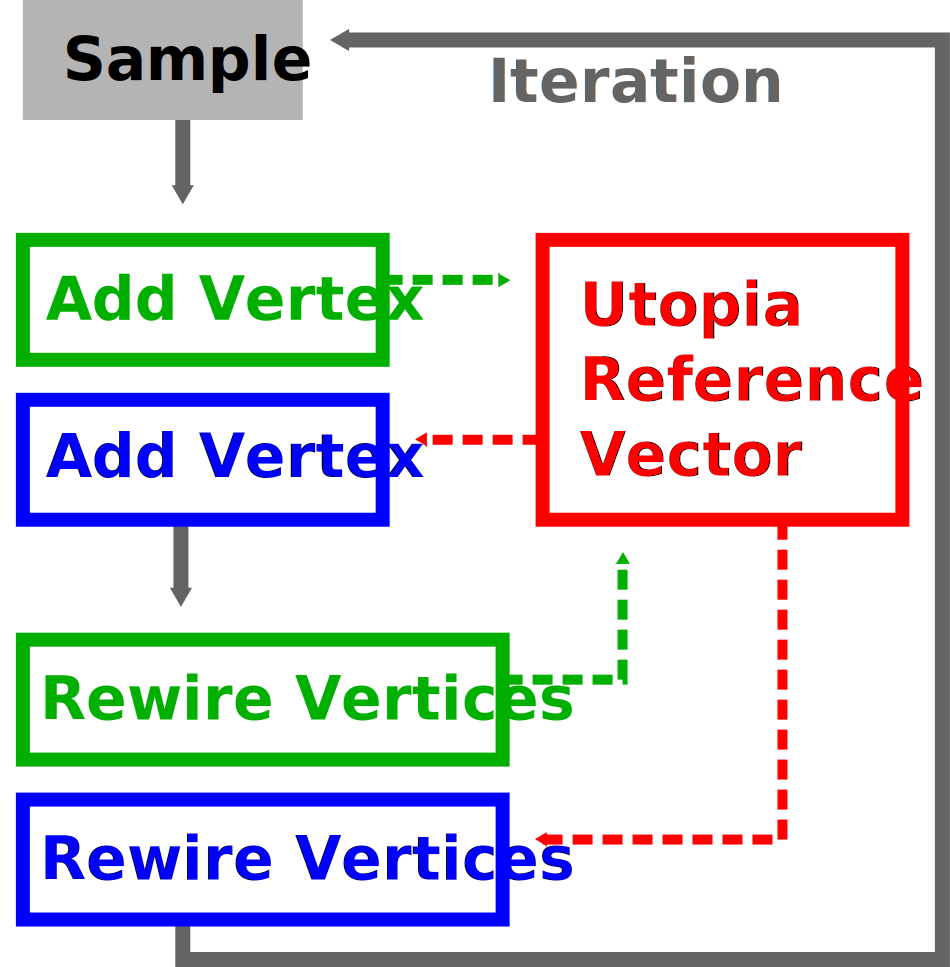
\includegraphics[width=.5\linewidth]{figure/MORRF_alg}
	\end{figure}
	
\end{frame}


\begin{frame}{Approaches}{Multi-Objective Path-Planning}
	
	\begin{columns}
		\column{.33\textwidth}
		\begin{block}{Weighted-Sum Approach}
		\begin{figure}[t]
			\centering
			\includegraphics[width=\linewidth]{figure/MORRF_weighted_sum}
		\end{figure}
	    \end{block}
		\column{.33\textwidth}
		\begin{block}{Tchebycheff Approach}
		\begin{figure}[t]
			\centering
			\includegraphics[width=\linewidth]{figure/MORRF_tchebycheff}
		\end{figure}
	    \end{block}
		\column{.33\textwidth}
		\begin{block}{Boundary-Intersection Approach}
		\begin{figure}[t]
			\centering
			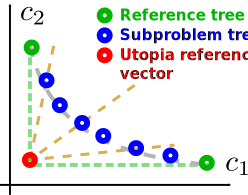
\includegraphics[width=\linewidth]{figure/MORRF_boundary_intersection}
		\end{figure}
    	\end{block}
	\end{columns}
	
\end{frame}

\begin{comment}
\begin{frame}{Weighted-Sum Approach}{Multi-Objective Path-Planning}

	{\bf Weighted-Sum Approach}
	
	\begin{columns}
		\column{0.4\textwidth}
		\begin{figure}[t]
			\centering
			\includegraphics[width=\linewidth]{figure/MORRF_weighted_sum}
		\end{figure}
		\column{0.57\textwidth}
		
        \begin{block}{}
		\begin{equation}
		\nonumber
		\arg\min_x \sum_{k=1}^{K} \lambda_{k} c_{k} (x)
		\end{equation}
		\end{block}

		
		\footnotesize{
			\begin{itemize}
			    \item Each reference tree returns a solution of one objective.
				\item Each subproblem tree returns a solution of weighted sum of all the objectives.
			\end{itemize}
		}
	\end{columns}
	
\end{frame}

\begin{frame}{Tchebycheff Approach}{Multi-Objective Path-Planning}
	{\bf Tchebycheff Approach}
	\begin{columns}
		\column{0.4\textwidth}
		\begin{figure}[t]
			\centering
			\includegraphics[width=\linewidth]{figure/MORRF_tchebycheff}
		\end{figure}
		\column{0.57\textwidth}
		
        \begin{block}{}
		\begin{equation}
		\nonumber
		\arg\min_x\max_{1 \leq k \leq K}  \{ \lambda_{k} | c_{k}(x) - \bm{z}^{\rm utop}_{k}  | \}
		\end{equation}
		\end{block}

		
		\footnotesize{
			\begin{itemize}
				\item Each reference tree adds a new vertex.
				\item Support the Utopia reference vector of the new position.
				\item According to the estimated Utopia reference vector, each subproblem tree adds a new vertex correspondingly.
			\end{itemize}
		}
	\end{columns}
\end{frame}

\begin{frame}{Boundary-Intersection Approach}{Multi-Objective Path-Planning}
	{\bf Boundary-Intersection Approach}
	\begin{columns}
		\column{0.4\textwidth}
		\begin{figure}[t]
			\centering
			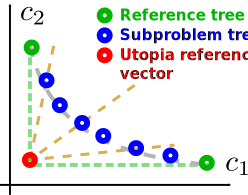
\includegraphics[width=\linewidth]{figure/MORRF_boundary_intersection}
		\end{figure}
		\column{0.57\textwidth}
		
        \begin{block}{}
		\begin{equation}
		\nonumber
		\arg\min_x \{ d \mid \bm{z}^{\rm utop} - c(x) = d \bm{\lambda} \} 
		\end{equation}
		\end{block}

		\footnotesize{
			\begin{itemize}
				\item Each reference tree rewires vertices near the new vertex.
				\item Support the Utopia reference vector of the rewired positions.
				\item According to the estimated Utopia reference vector, each subproblem tree rewires vertices near the new vertex correspondingly.
			\end{itemize}
		}
	\end{columns}
\end{frame}
\end{comment}

\subsection{Validation}

\begin{frame}{Validation - Theoretical Analysis}{Multi-Objective Path-Planning}

\begin{thm}
	The solutions generated by MORRF$^{*}$ \textcolor{blue}{converge} to \textcolor{red}{a subset of the Pareto optimal set}
	\textcolor{blue}{almost surely}.
\end{thm}

\begin{columns}
\column{0.45\textwidth}
	\begin{figure}
		\centering
		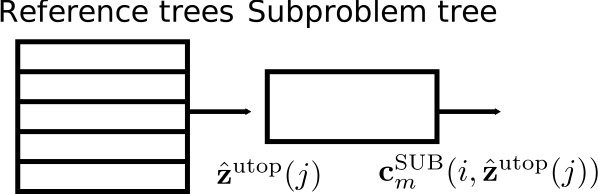
\includegraphics[width=.8\linewidth]{figure/cascade}
	\end{figure}
\column{0.45\textwidth}
	\begin{figure}
		\centering
		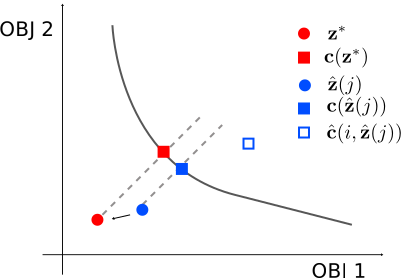
\includegraphics[width=.8\linewidth]{figure/conv}
	\end{figure}
\end{columns}	
	
\end{frame}

\begin{frame}{Validation - Simulation}{Multi-Objective Path-Planning}

\begin{columns}
\column{0.32\textwidth}
	\begin{figure}
		\centering
		\includegraphics[width=\linewidth]{figure/sim2-2obj/MORRTstar00-0}
	\end{figure}
\column{0.32\textwidth}
	\begin{figure}
		\centering
		\includegraphics[width=\linewidth]{figure/sim2-2obj/MORRTstar00-1}
	\end{figure}
\column{0.35\textwidth}
\begin{block}{Process}
\begin{itemize}
\item Different cost function
\item Parallel exploration
\end{itemize}
\end{block}		
\end{columns}

\begin{columns}
\column{0.32\textwidth}
	\begin{figure}
		\centering
		\includegraphics[width=\linewidth]{figure/sim2-2obj/MORRTstar00-ALL}
	\end{figure}
\column{0.32\textwidth}
	\begin{figure}
		\centering
		\includegraphics[width=\linewidth]{figure/sim2-2obj/PF02-MORRT2}
	\end{figure}
\column{0.35\textwidth}	
\begin{block}{Performance}
\begin{itemize}
\item Pareto optimality
\item Solution diversity
\end{itemize}
\end{block}	
\end{columns}
	
\end{frame}


\begin{frame}{Validation - Simulation}{Multi-Objective Path-Planning}

\begin{columns}[t]

\column{0.32\textwidth}
\begin{block}{Approaches}
\begin{itemize}
\item NSGA-II
\item Weighted-Sum Approach
\item Tchebycheff Approach
\item Boundary-Intersection Approach
\end{itemize}
\end{block}

\column{0.32\textwidth}
\begin{block}{Environment}
\begin{itemize}
\item Non-Obstacle
\item Obstacle
\end{itemize}
\end{block}

\column{0.32\textwidth}
\begin{block}{Objectives}
\begin{itemize}
\item Two objectives
\item Three objectives
\item Non-convex objectives
\end{itemize}
\end{block}

\end{columns}

\end{frame}


\section{Topological Preference in Path-Planning}

% add outline page with current section highlighted.
\begin{frame}{Outline}{ $ \null $ }
	\tableofcontents[currentsection]
	%\tableofcontents[currentsection,currentsubsection]
\end{frame}

\subsection{Path-Planning with Reference Path}

\subsubsection{Algorithm}

\begin{frame}{Coverage Model in Path-Planning}{Path-Planning with Reference Path}

\begin{itemize}
\item Information measurement - entropy 
\item Maximum coverage problem
\end{itemize}

\begin{figure}
\centering
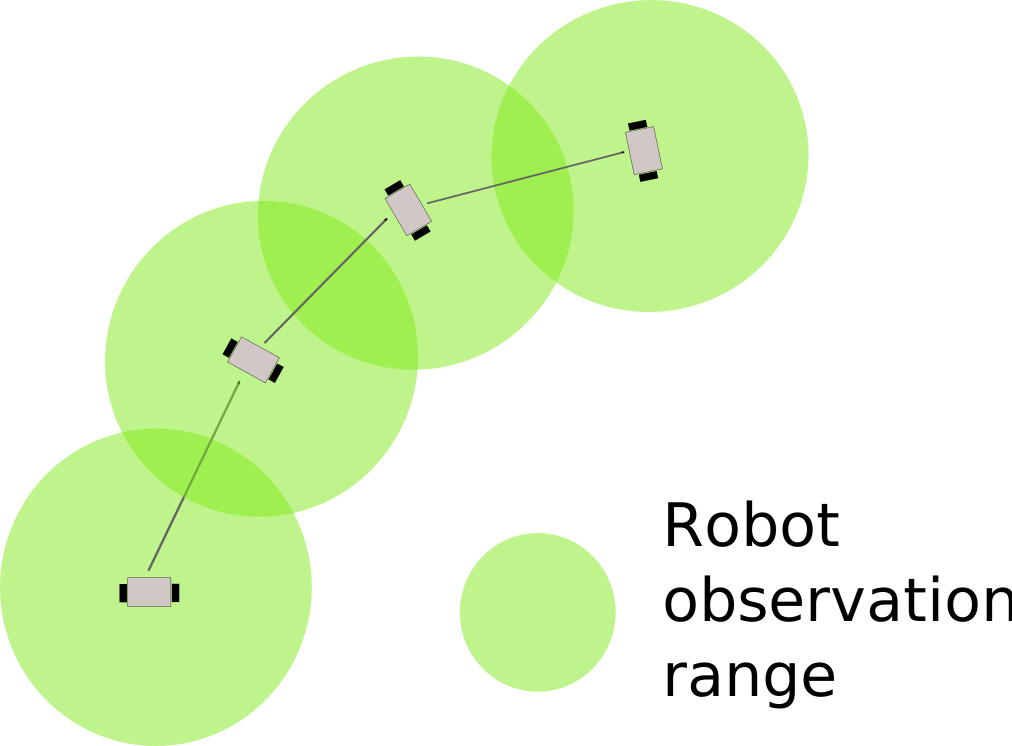
\includegraphics[width = 0.6\textwidth]{./figure/robotObservation}
\end{figure}

\end{frame}

\begin{comment}
\begin{frame}{Submodularity}{Path-Planning with Reference Path}

\begin{columns}

\column{0.45\textwidth}

\begin{figure}
\centering
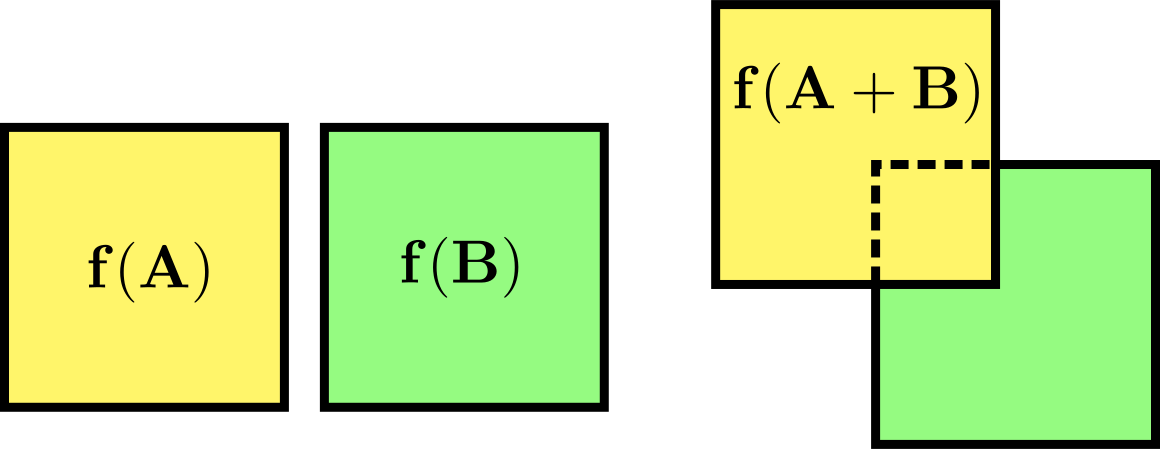
\includegraphics[width = \textwidth]{./figure/submodular}
%\caption{A coverage model.}
\end{figure}

\begin{equation}
\nonumber
f(A) + f(B) \geq f(A+B)
\end{equation}

\column{0.1\textwidth}

\column{0.45\textwidth}

Information
\begin{itemize}
\item search space $ S $
\item the observation of a robot $ \mathbf{O}^{X} $ 
\item the observation of a human $ \mathbf{O}^{Y} $

\bigskip
\bigskip

$ f( \mathbf{S}, \mathbf{O}^{X} ) + f( \mathbf{S}, \mathbf{O}^{Y^{h}} ) \geq f( \mathbf{S}, \mathbf{O}^{X},  \mathbf{O}^{Y^{h}} ) $ 
\end{itemize}

\end{columns}

\end{frame}

\begin{frame}{Submodular orienteering}{Path-Planning with Reference Path}

\begin{block}{Conditional mutual information}
$ I(\mathbf{S}; \mathbf{O}^{X} \mid \mathbf{O}^{Y^{h}}) = H(\mathbf{S} \mid \mathbf{O}^{Y^{h}}) - H(\mathbf{S} \mid \mathbf{O}^{X},\mathbf{O}^{Y^{h}}) $
\end{block} 

\bigskip

\begin{itemize}
\item Entropy reduction
\item Submodularity
\item Chain rule \\
$ I(\mathbf{S}; \mathbf{O}^{X} \mid \mathbf{O}^{Y^{h}}) = \sum_{t=1}^{T} I(O^{X}_{t} ; \mathbf{S} \mid O^{X}_{1} , \cdots , O^{X}_{t-1}, \mathbf{O}^{Y^{h}}) $
\end{itemize}

\end{frame}
\end{comment}

\begin{frame}{Human Constraint}{Path-Planning with Reference Path}

\begin{figure}
\centering
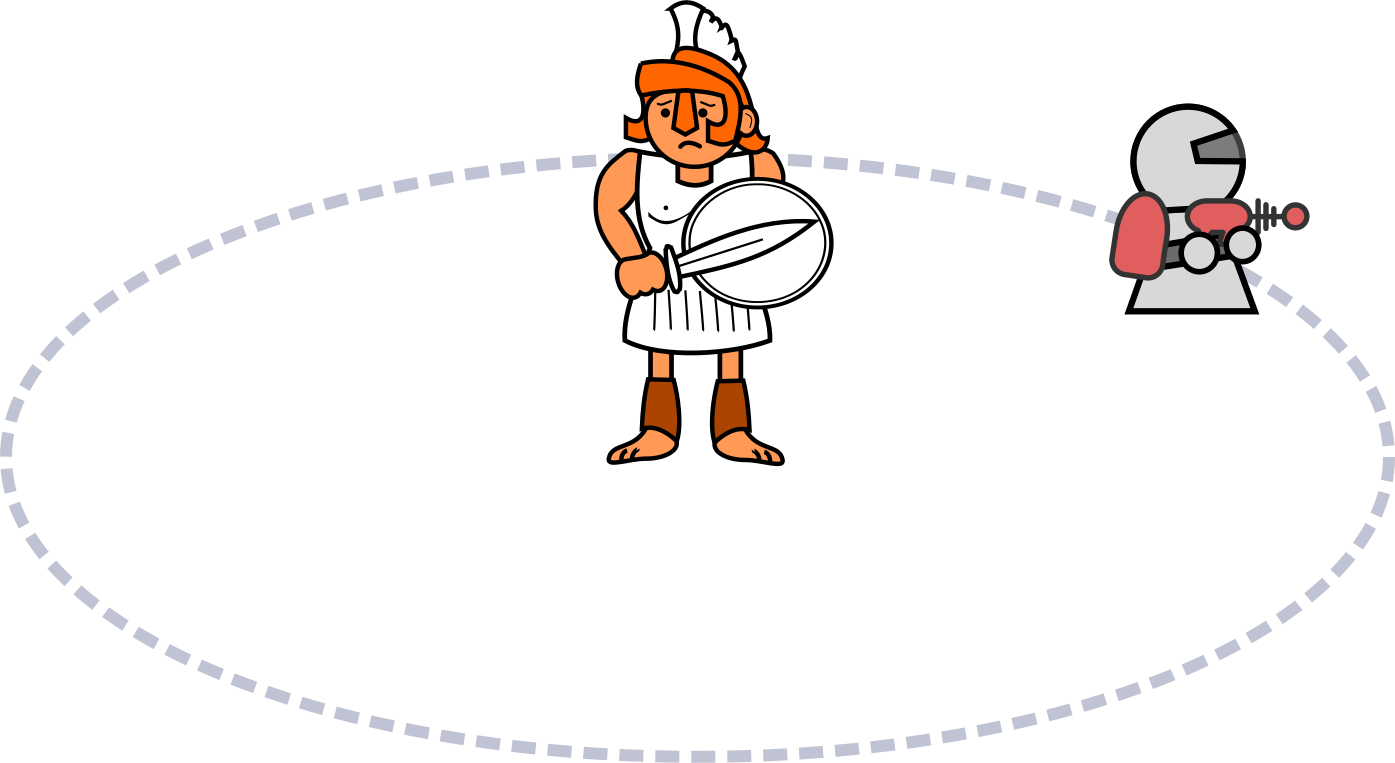
\includegraphics[width = 0.7\textwidth]{./figure/human_robot_interaction}
\end{figure}

\begin{itemize}
\item cooperative observation
\item assistance and protection
\end{itemize}

\end{frame}

\begin{frame}{Neighboring Function}{Path-Planning with Reference Path}

\begin{columns}
\column{.6\linewidth}
\begin{minipage}[c]{\linewidth}
\begin{figure}
\centering
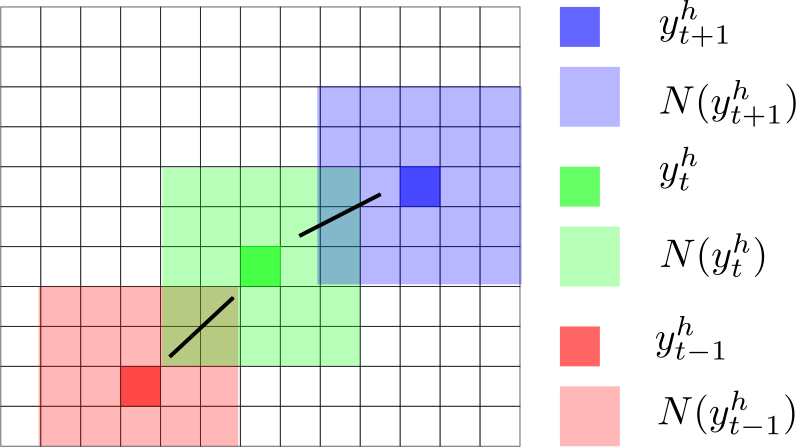
\includegraphics[width = \textwidth]{./figure/humanConstraint}
\end{figure}
\end{minipage}

\column{.4\linewidth}
\begin{minipage}[c]{\linewidth}
\begin{itemize}
\item { human path $ \{ y^{h}_{1} \cdots y^{h}_{T} \} $ }
\item { neighboring function $ N( y^{h}_{t} ) $ }
\end{itemize}
\end{minipage}
\end{columns}

\end{frame}

\begin{frame}{Reference Path}{Path-Planning with Reference Path}

\begin{figure}
\centering
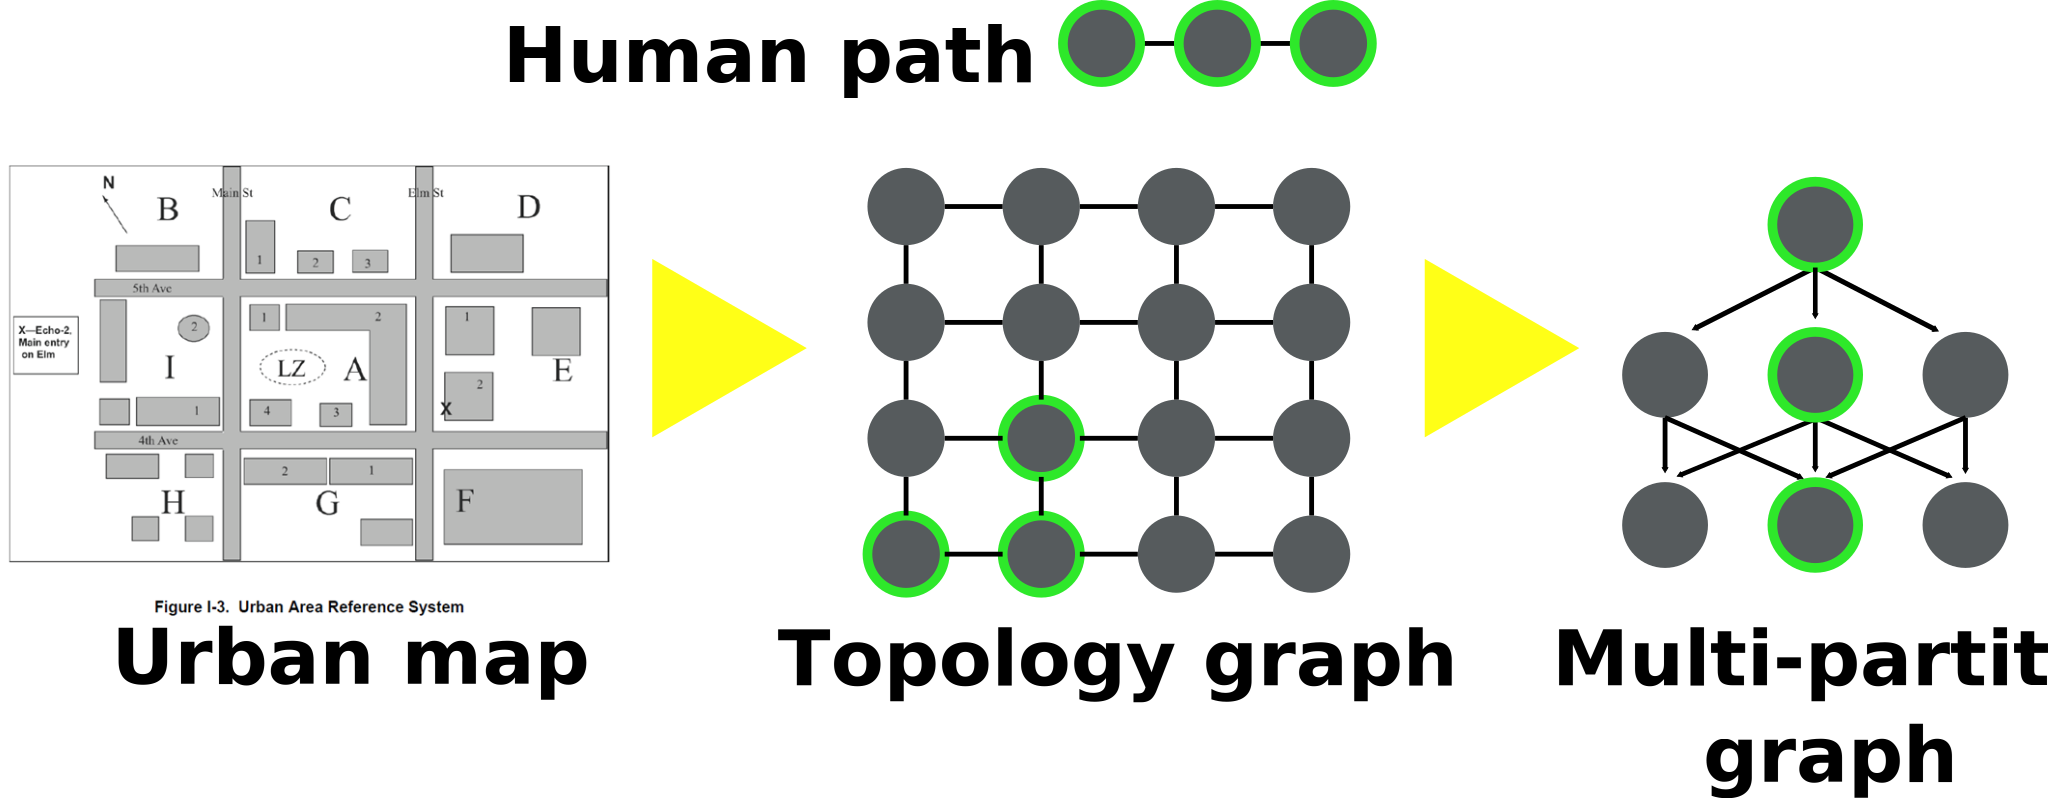
\includegraphics[width = 0.9\textwidth]{./figure/layers}
\end{figure}

\end{frame}

\begin{frame}{The Multi-Partite Graph}{Path-Planning with Reference Path}

\begin{columns}

\column{.6\textwidth}
\begin{minipage}[c]{\textwidth}
\begin{figure}
\centering
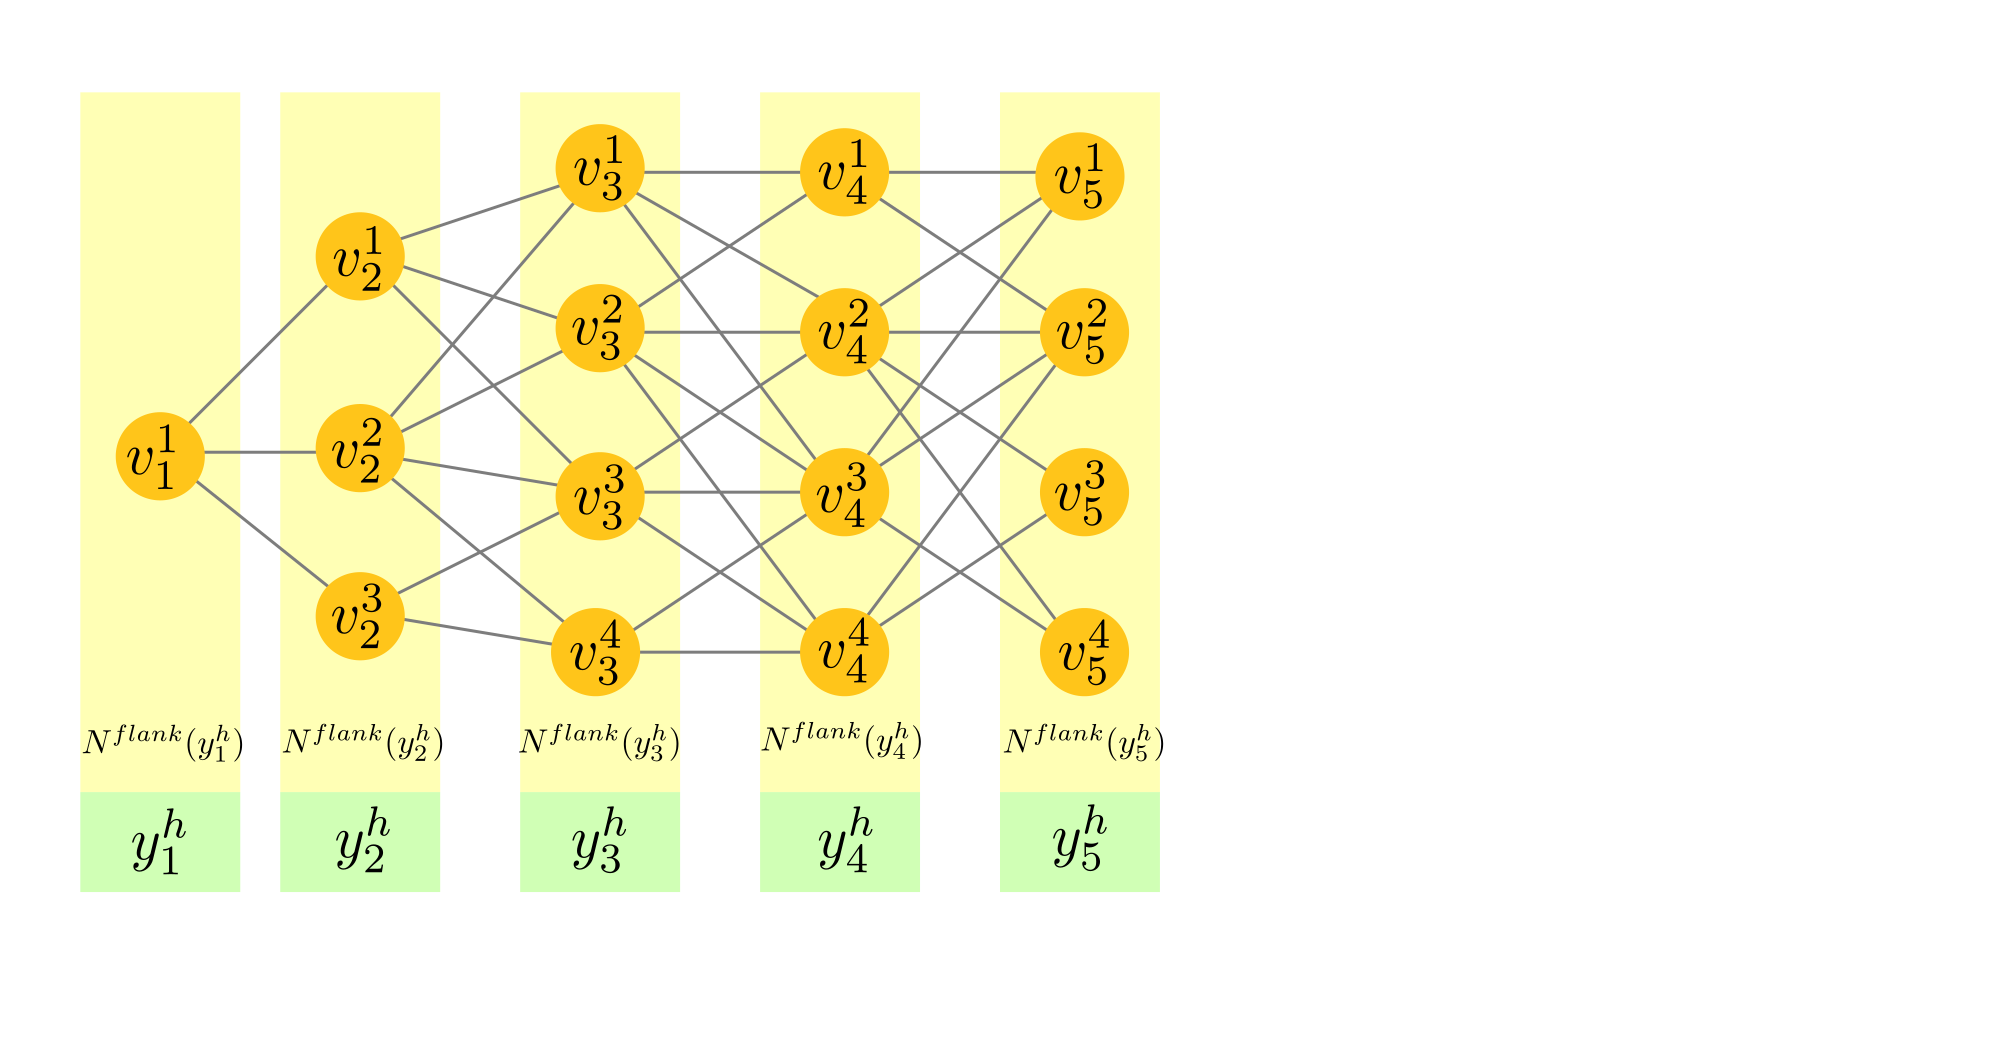
\includegraphics[width = .8\textwidth]{./figure/MultiPartite}
\end{figure}
\end{minipage}

\column{.4\textwidth}
\begin{minipage}[c]{\textwidth}
\begin{itemize}
\item time-space synchronization
\item connection determined by discretized map
\end{itemize}
\end{minipage}

\end{columns}

\begin{block}{Submodular Orienteering on a Multi-Partite Graph}
\begin{equation}
\nonumber
\begin{aligned}
Objective: & X^{*} = \argmax_{X} \: f(X); \\
Constraint: & |X| = T, x_{t} \in V(t), (x_{t}, x_{t+1}) \in E.
\end{aligned}
\end{equation}
\end{block}

\end{frame}

\begin{frame}{A Pruning Process}{Path-Planning with Reference Path}

\begin{columns}

\column{.47\textwidth}
\begin{block}{Forward Pruning}
Reachable 
\begin{columns}
\column{.15\textwidth}
\column{.4\textwidth}
\tiny{
\noindent
$ \forall t \in \{ 2, \cdots T \}, $ \\
$ \forall v \in V(t), $  \\
$ deg^{-}(v) > 0 $
}
\column{.3\textwidth}
\begin{figure}
\centering
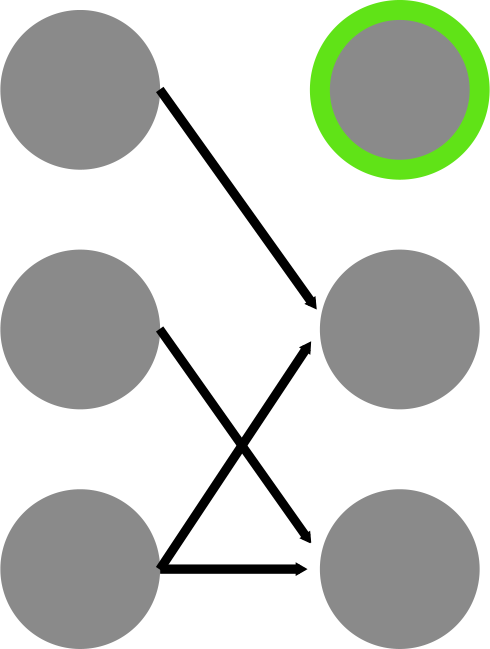
\includegraphics[width = \textwidth]{./figure/forward_prune}
\end{figure}
\column{.15\textwidth}
\end{columns}
\end{block}

\column{.47\textwidth}

\begin{block}{Backward Pruning}
Non-terminating 
\begin{columns}
\column{.15\textwidth}
\column{.4\textwidth}
\tiny{
\noindent
$ \forall t \in \{ 1, \cdots T-1 \}, $ \\
$ \forall v \in V(t), $ \\ 
$ deg^{+}(v) > 0 $
}
\column{.3\textwidth}
\begin{figure}
\centering
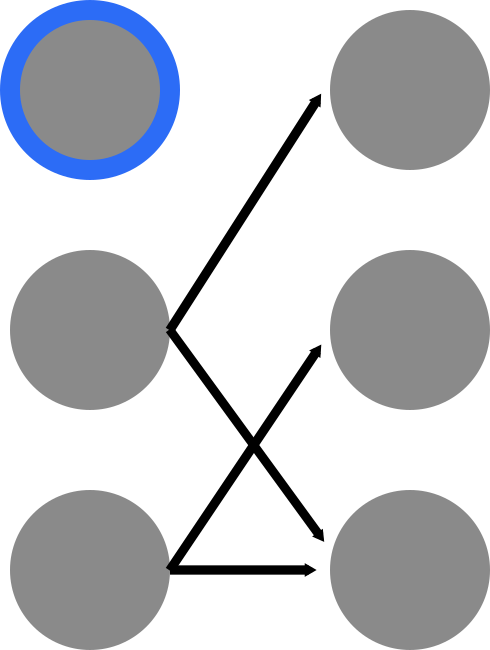
\includegraphics[width = \textwidth]{./figure/backward_prune}
\end{figure}
\column{.15\textwidth}
\end{columns}
\end{block}

\end{columns}

\begin{block}{Obstacles}
\begin{figure}
\centering
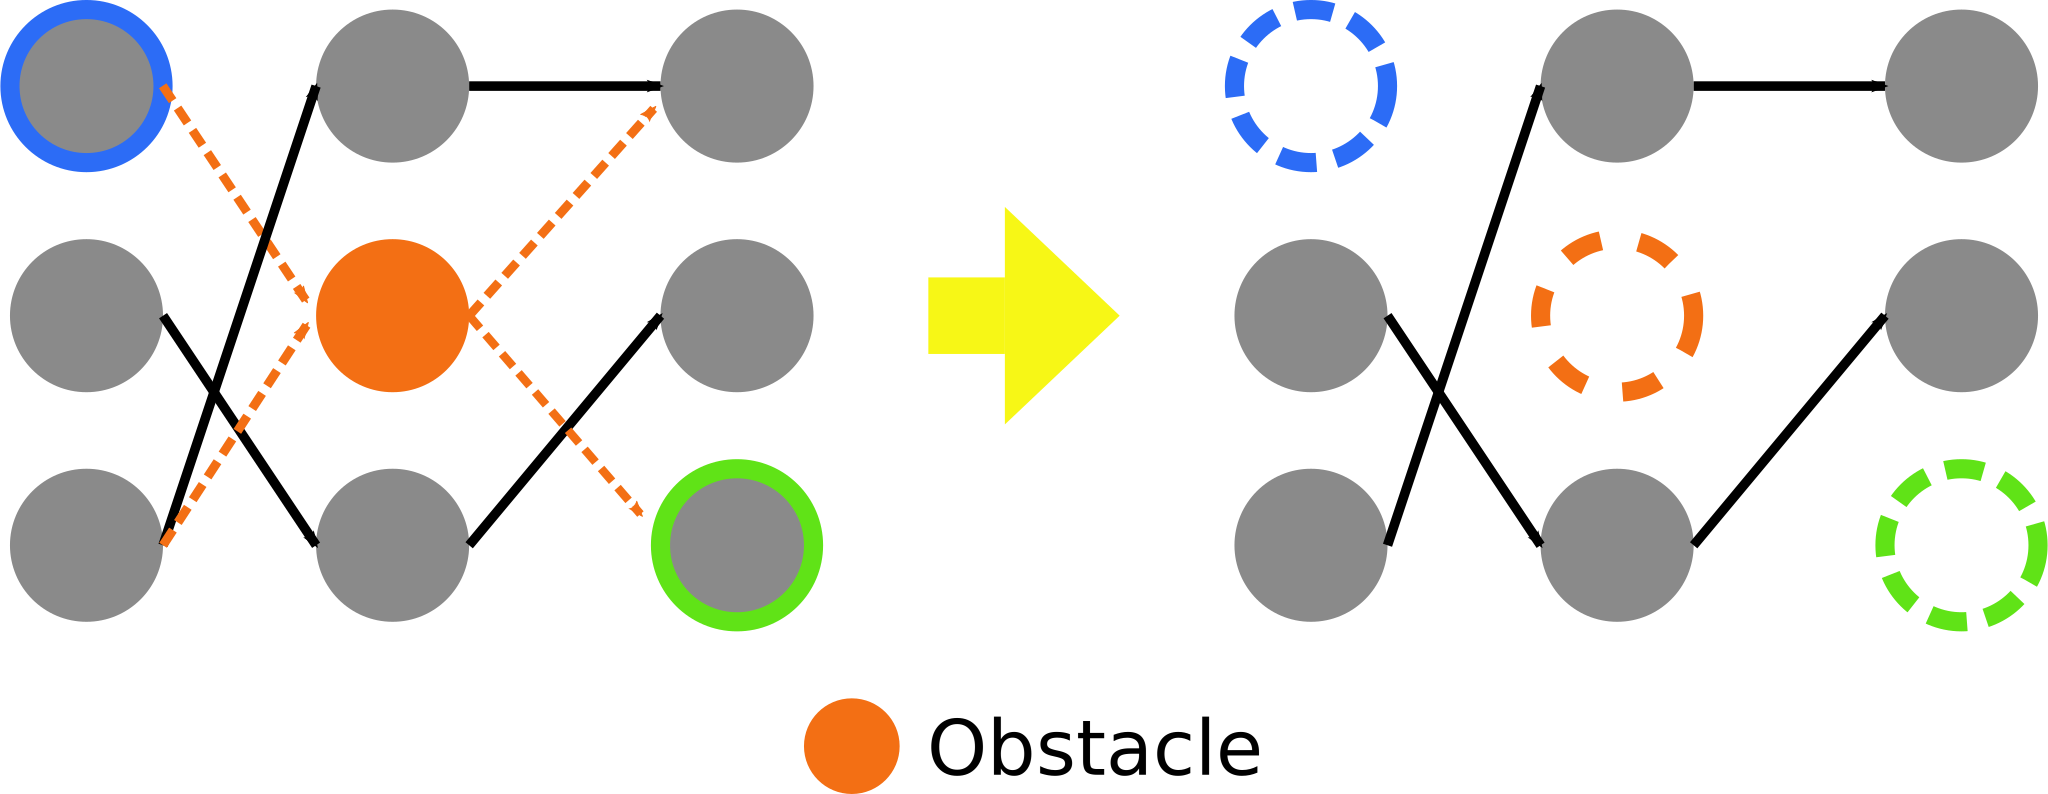
\includegraphics[width = 0.5\textwidth]{./figure/obstacle}
\end{figure}
\end{block}

\end{frame}

\begin{frame}{Algorithms}{Path-Planning with Reference Path}

\begin{columns}

\column{0.5\textwidth}
\begin{minipage}{\textwidth}
\begin{block}{Backtracking Heuristic}
\begin{figure}
\centering
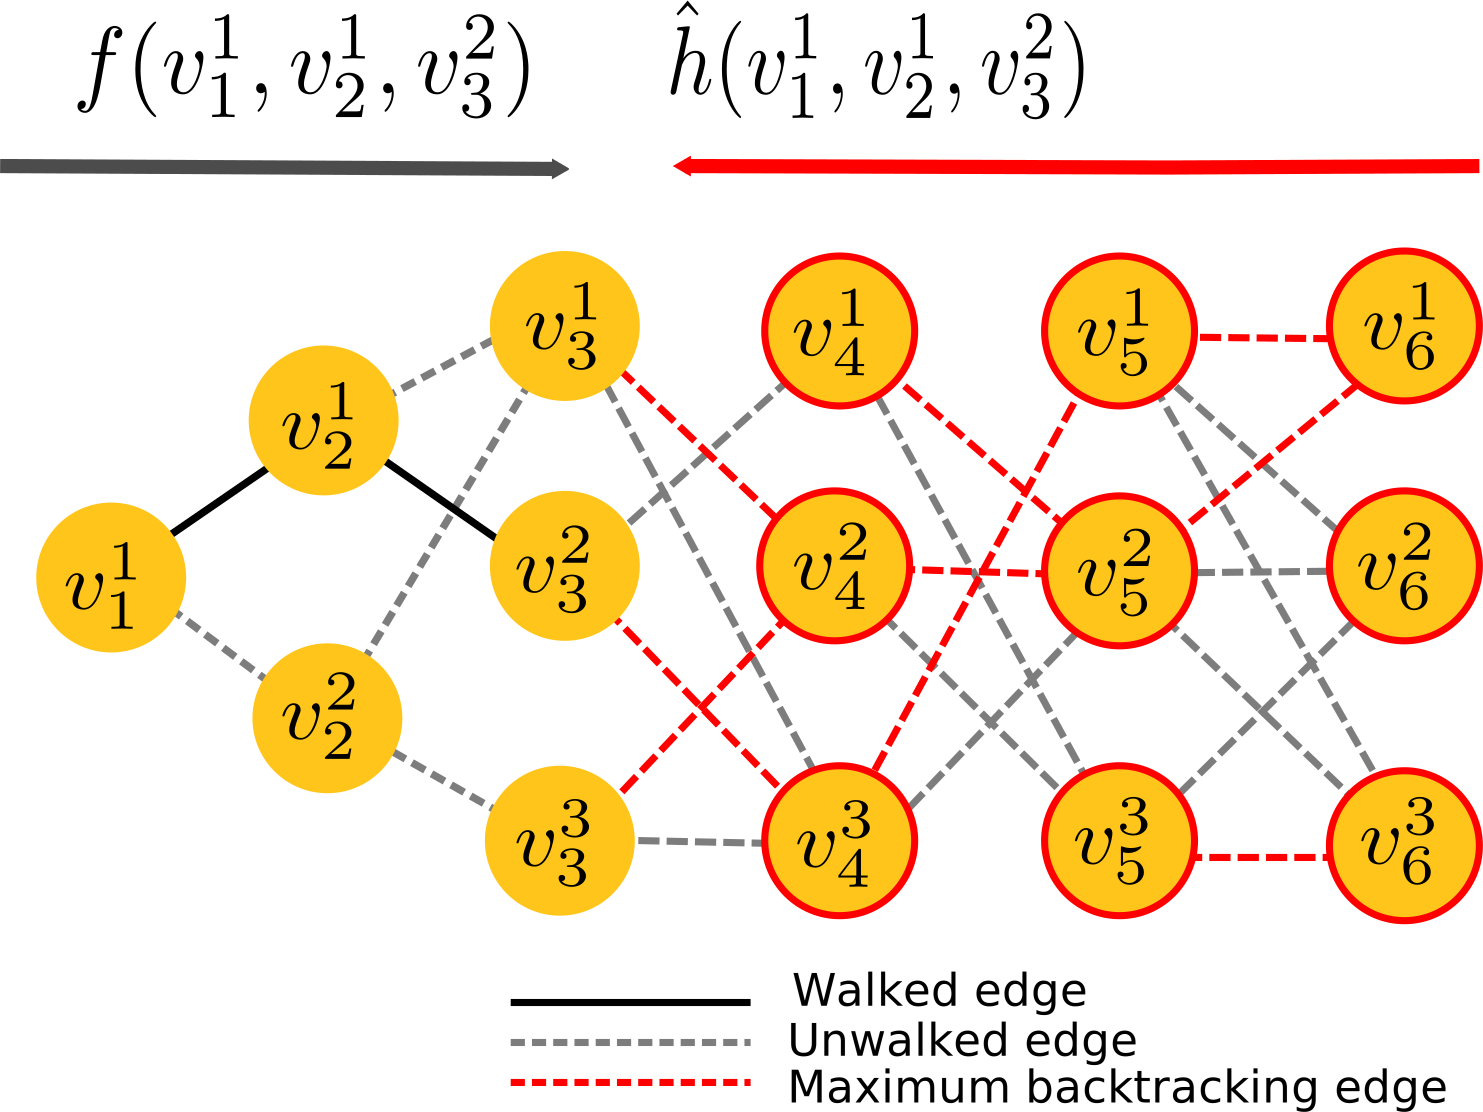
\includegraphics[width = .7\textwidth]{./figure/backtracking}
\end{figure}
\end{block}
\end{minipage}

\column{0.4\textwidth}
\begin{minipage}{\textwidth}
\begin{block}{Expanding Tree}
\begin{figure}
\centering
\includegraphics[width = .7\textwidth]{./figure/multipartite_expandingtree}
\end{figure}
\end{block}
\end{minipage}

\end{columns}

\centering
\begin{minipage}{.6\textwidth}
\begin{block}{Node Freeze}
\begin{figure}
\centering
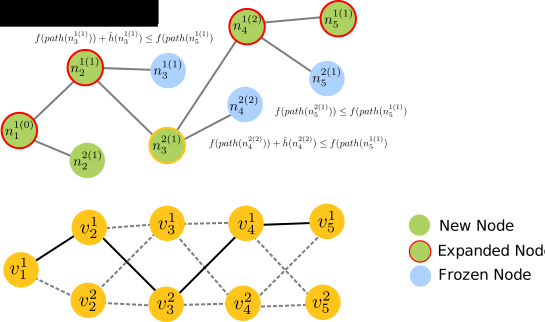
\includegraphics[width = \textwidth]{./figure/freeze_process}
\end{figure}
\end{block}
\end{minipage}

\end{frame}

\begin{frame}{Anytime Algorithm Framework}{Path-Planning with Reference Path}

\begin{figure}
\centering
\includegraphics[width = 0.9\textwidth]{./figure/alg_flow}
\end{figure}

\end{frame}

\subsubsection{Validation}

\begin{frame}{Validation - Theoretical Analysis}{Path-Planning with Reference Path}

\begin{lemma}
Backtracking never \textcolor{red}{underestimates}
the maximum total reward, which means
\begin{equation}
\nonumber
\forall t \geq t', \hat{u}(x_{t} \mid v_{1} , \cdots , v_{t'}) \geq u(x_{t} \mid v_{1} , \cdots , v_{t'}).
\end{equation}
\end{lemma}

\begin{minipage}{\textwidth}
\begin{figure}
\centering
\includegraphics[width = 0.15\textwidth]{./figure/arrow}
\end{figure}
\end{minipage}

\begin{theorem}
The anytime algorithm framework can always find an \textcolor{red}{optimal} solution given enough time.
\end{theorem}

\end{frame}

\begin{frame}{Validation - Simulation}{Path-Planning with Reference Path}

{\bf Robot Wingman}

\begin{figure}
\centering
\includegraphics[width = .35\textwidth]{./figure/Wingman}
\end{figure}

\begin{columns}

\column{0.25\textwidth}
\begin{minipage}{\textwidth}
\begin{block}{Path planning}
\centering
\includegraphics[width = \textwidth]{./figure/simulation/hexamap.png}
\end{block}
\end{minipage}

%\column{0.1\textwidth}
%\begin{minipage}{\textwidth}
%\centering
%\includegraphics[width = \textwidth]{./figure/arrow2}
%\end{minipage}

\column{0.25\textwidth}
\begin{minipage}{\textwidth}
\begin{block}{Waypoints}
\centering
\includegraphics[width = \textwidth]{./figure/simulation/waypoint.png}
\end{block}
\end{minipage}

%\column{0.1\textwidth}
%\begin{minipage}{\textwidth}
%\centering
%\includegraphics[width = \textwidth]{./figure/arrow2}
%\end{minipage}

\column{0.4\textwidth}
\begin{minipage}{\textwidth}
\begin{block}{Robot execution}
\centering
\includegraphics[width = \textwidth]{./figure/simulation/gazebo2.png}
\end{block}
\end{minipage}

\end{columns}

\end{frame}

\begin{frame}{Validation - Simulation}{Path-Planning with Reference Path}

\begin{columns}

\column{0.3\textwidth}
\begin{minipage}{\textwidth}
\begin{block}{quality of heuristic}
{\small 
\textcolor{metric-OFI}{Percentage of optimal at first iteration}
}
\end{block}
\end{minipage}

\column{0.7\textwidth}
\begin{figure}
\includegraphics[width=\textwidth]{./figure/metric2}
\end{figure}

\end{columns}

\begin{columns}

\column{0.3\textwidth}

\column{0.7\textwidth}
\begin{center}
\begin{minipage}{0.43\textwidth}
\begin{block}{quality of algorithm}
{\small 
\textcolor{metric-IRO}{Number of iterations to reach optimal (normalized)}
}
\end{block}
\end{minipage}
\end{center}

\end{columns}

\end{frame}

\begin{frame}{Validation - Simulation}{Path-Planning with Reference Path}

\begin{columns}[t]

\column{0.32\textwidth}
\begin{block}{Heuristic}
\begin{itemize}
\item greedy heuristic 
\item backtracking heuristic
\end{itemize}
\end{block}

\column{0.32\textwidth}
\begin{block}{Environment}
\begin{itemize}
\item Uniform
\item Random	
\item Multi-Modal
\end{itemize}
\end{block}

\column{0.32\textwidth}
\begin{block}{Reference Paths}
\begin{itemize}
\item Line
\item Spiral
\item Lawn-mower
\item Arc
\item Loitering
\end{itemize}
\end{block}

\end{columns}

\end{frame}





\subsection{Homotopy-based Path-Planning}

\subsubsection{Algorithm}

\begin{frame}{Homotopy in Path-Planning}{Homotopy-based Path-Planning}
	
\begin{columns}
\column{.45\textwidth}
\begin{figure}
	\centering
	\begin{subfigure}
		\centering
		\includegraphics[width=.47\textwidth]{figure/all_homotopy_classes/s1.png}
	\end{subfigure}  
	\begin{subfigure}
		\centering
		\includegraphics[width=.47\textwidth]{figure/all_homotopy_classes/s2.png}
	\end{subfigure}
	\\
	\begin{subfigure}
		\centering
		\includegraphics[width=.47\textwidth]{figure/all_homotopy_classes/s3.png}
	\end{subfigure}  
	\begin{subfigure}
		\centering
		\includegraphics[width=.47\textwidth]{figure/all_homotopy_classes/s4.png}
	\end{subfigure}
	\\
	\begin{subfigure}
		\centering
		\includegraphics[width=.47\textwidth]{figure/all_homotopy_classes/s5.png}
	\end{subfigure}	 
	\begin{subfigure}
		\centering
		\includegraphics[width=.47\textwidth]{figure/all_homotopy_classes/s6.png}
	\end{subfigure}	 
\end{figure}
\column{.52\textwidth}
\begin{block}{Hard Constraint}
\begin{itemize}
\item Specific homotopy class
\item Via-regions / Forbidden regions
\end{itemize}
\end{block}
\begin{block}{Soft Constraint}
\begin{itemize}
\item Homotopy preference
\end{itemize}
\end{block}
\end{columns}
	
\end{frame}

\begin{frame}{Homotopy-based Optimal Path-Planning}{Homotopy-based Path-Planning}
	
\begin{columns}
\column{.45\textwidth}
\begin{figure}
	\centering
	\begin{subfigure}
		\centering
		\includegraphics[width=.47\textwidth]{figure/all_homotopy_classes/s1.png}
	\end{subfigure}  
	\begin{subfigure}
		\centering
		\includegraphics[width=.47\textwidth]{figure/all_homotopy_classes/s2.png}
	\end{subfigure}
	\\
	\begin{subfigure}
		\centering
		\includegraphics[width=.47\textwidth]{figure/all_homotopy_classes/s3.png}
	\end{subfigure}  
	\begin{subfigure}
		\centering
		\includegraphics[width=.47\textwidth]{figure/all_homotopy_classes/s4.png}
	\end{subfigure}
	\\
	\begin{subfigure}
		\centering
		\includegraphics[width=.47\textwidth]{figure/all_homotopy_classes/s5.png}
	\end{subfigure}	 
	\begin{subfigure}
		\centering
		\includegraphics[width=.47\textwidth]{figure/all_homotopy_classes/s6.png}
	\end{subfigure}	 
\end{figure}
\column{.52\textwidth}
\begin{block}{Optimal Paths of Homotopy Classes}
\begin{itemize}
\item $ \bm{H} ( x_{init}, x_{goal} ) $ - the set of homotopy classes defined by $ x_{init} $ and $ x_{goal} $
\item $ H = { h_1 , \cdots , h_N } \subseteq \bm{H} $
\item $ \forall h_i \in H, \sigma^{*}_{h_i} = \arg \min_{\sigma \in X_{\it free} \land h(\sigma) = h_i } \mbox{\sc Cost}  (\sigma) $
\end{itemize}
\end{block}
\end{columns}
	
\end{frame}

\begin{frame}{Homotopy-based Optimal Path-Planning}{Homotopy-based Path-Planning}

{\bf Solution}

\begin{block}{}
Convert a path into a string representation
\end{block}
\begin{block}{}
Determine the homotopic equivalence by string representation
\end{block}
\begin{block}{}
Find the optimal paths by string representation
\end{block}

\end{frame}

\begin{frame}{Generate String Representation}{Homotopy-based Path-Planning}

\begin{columns}

\column{.4\textwidth}
\begin{figure}
	\centering
	\includegraphics[width=\linewidth]{figure/obs_map}
\end{figure}
\column{.57\textwidth}
\begin{itemize}
\item A ray structure decomposes the map
\item Reference frames with ID
\item How a path sequentially crosses reference frames generates a string of IDs
\end{itemize}
\end{columns}

\end{frame}

\begin{frame}{Homotopy Equivalence}{Homotopy-based Path-Planning}

\begin{columns}

\column{.33\textwidth}
\begin{figure}
	\centering
	\includegraphics[width=\linewidth]{figure/obs_topology}
\end{figure}
\column{.05\textwidth}
\begin{figure}
	\centering
	\includegraphics[width=\linewidth]{figure/arrow2}
\end{figure}
\column{.3\textwidth}
\begin{figure}
	\centering
	\includegraphics[width=\linewidth]{figure/equivalence1}
\end{figure}
\begin{figure}
	\centering
	\includegraphics[width=\linewidth]{figure/equivalence2}
\end{figure}
\column{.05\textwidth}
\begin{figure}
	\centering
	\includegraphics[width=\linewidth]{figure/arrow2}
\end{figure}
\column{.18\textwidth}
\begin{figure}
	\centering
	\includegraphics[width=\linewidth]{figure/obs_topology2}
\end{figure}
\end{columns}

\end{frame}

\begin{frame}{Homotopy-Aware Optimal Search}{Homotopy-based Path-Planning}

\begin{columns}

\column{.33\textwidth}
\begin{block}{RRT*}
\begin{figure}
	\centering
	\includegraphics[width=\linewidth]{figure/single_tree}
\end{figure}
\end{block}
\column{.33\textwidth}
\begin{block}{Bi-RRT*}
\begin{figure}
	\centering
	\includegraphics[width=\linewidth]{figure/bi_tree}
\end{figure}
\end{block}
\column{.33\textwidth}
\begin{block}{RRG*}
A graph structure
\begin{figure}
	\centering
	\includegraphics[width=.5\linewidth]{figure/question_mark}
\end{figure}
\end{block}
\end{columns}

\end{frame}

\subsubsection{Validation}

\begin{frame}{Validation - Theoretical Analysis}{Homotopy-based Path-Planning}
	
{\bf The Mapping between Homotopy Classes and String Blocks}

\begin{figure}
	\centering
	\includegraphics[width=.7\linewidth]{figure/decomp_hierarchy}
\end{figure}

\begin{thm}
${\rm REPTrim}(\bm{M}^h(\sigma_i)) =  {\rm REPTrim}(\bm{M}^h(\sigma_j )) $\footnotemark
 iff $\sigma_i \simeq \sigma_j$.
\end{thm}	
	
\footnotetext[1]{ $ \bm{M}^h() $ is a DFA that converts a path into a string.}	
	
\end{frame}

\begin{frame}{Validation - Theoretical Analysis}{Homotopy-based Path-Planning}

\begin{thm}
The solutions of the proposed algorithm can find the optimal paths of all simple homotopy classes\footnotemark.
\end{thm}

\begin{itemize}
\item All the simple homotopy classes would be explored.
\item The solutions of all the simple homotopy classes converge to optimal.
\end{itemize}


\footnotetext[1]{{\bf Simple homotopy class} is defined as a homotopy class of paths that do not form complete loops around obstacles.}

\end{frame}

\begin{frame}{Validation - Simulation}{Homotopy-based Path-Planning}

\begin{columns}[t]

\column{0.32\textwidth}
\begin{block}{Optimal Search}
\begin{itemize}
\item RRT*
\item Bi-RRT*
\item RRG 
\end{itemize}
\end{block}

\column{0.32\textwidth}
\begin{block}{Environment}
\begin{itemize}
\item Simple obstacles
\item Complex obstacles
\end{itemize}
\end{block}

\column{0.32\textwidth}
\begin{block}{Constraint}
\begin{itemize}
\item Single Homotopy Class
\item Multiple Homotopy Classes
\end{itemize}
\end{block}

\end{columns}

\end{frame}




\begin{frame}{Schedule}{$ \null $}

\tiny

\begin{block}{}
\setbeamercolor{item}{fg=green}
\begin{itemize}
\item Toward Task-Based Mental Models of Human-Robot Teaming: A Bayesian Approach. (HCII 2013)
\item Supporting Task-oriented Collaboration in Human-Robot Teams using Semantic-based Path Planning. (DSS 2014)
\item Path Planning with a Human Path Constraint. (IEEE SMC 2014)
\item Input-to-State Stability Analysis on Particle Swarm Optimization. (GECCO 2015)
\item MORRF* : Sampling-based Multi-Objective Motion Planning. (IJCAI 2015)
\end{itemize}
\end{block}

\begin{block}{}
\setbeamercolor{item}{fg=yellow}
\begin{itemize}
\item Homotopy-Aware RRT* : Toward Human-Robot Topological Path-Planning. (HRI 2016, Submitted)
\end{itemize}
\end{block}

\begin{block}{}
\setbeamercolor{item}{fg=red}
\begin{itemize}
\item Understanding Adverbs in Natural Language Instructions : a Cost-Function Learning Approach (CDCG)
\item Understanding the Particle Swarm Optimization by Component Decomposition (PSO-ISS)
\item Toward Verbally Instructing Robot Navigation by Expressing Topological Constraint. (HDCG)
\item Sampling-based Multi-Objective Path Planning (MORRF*)
\item Finding the Optimal Path-Planning with Different Homotopy Classes (HARRT*)
\end{itemize}
\end{block}

\end{frame}

\begin{frame}{$ \null $}{$ \null $}

\centering
{\Large \bf Thank you!}

\end{frame}

\end{document}


